\documentclass{standalone}
\usepackage{tikz}
\usetikzlibrary{patterns, positioning}

\begin{document}
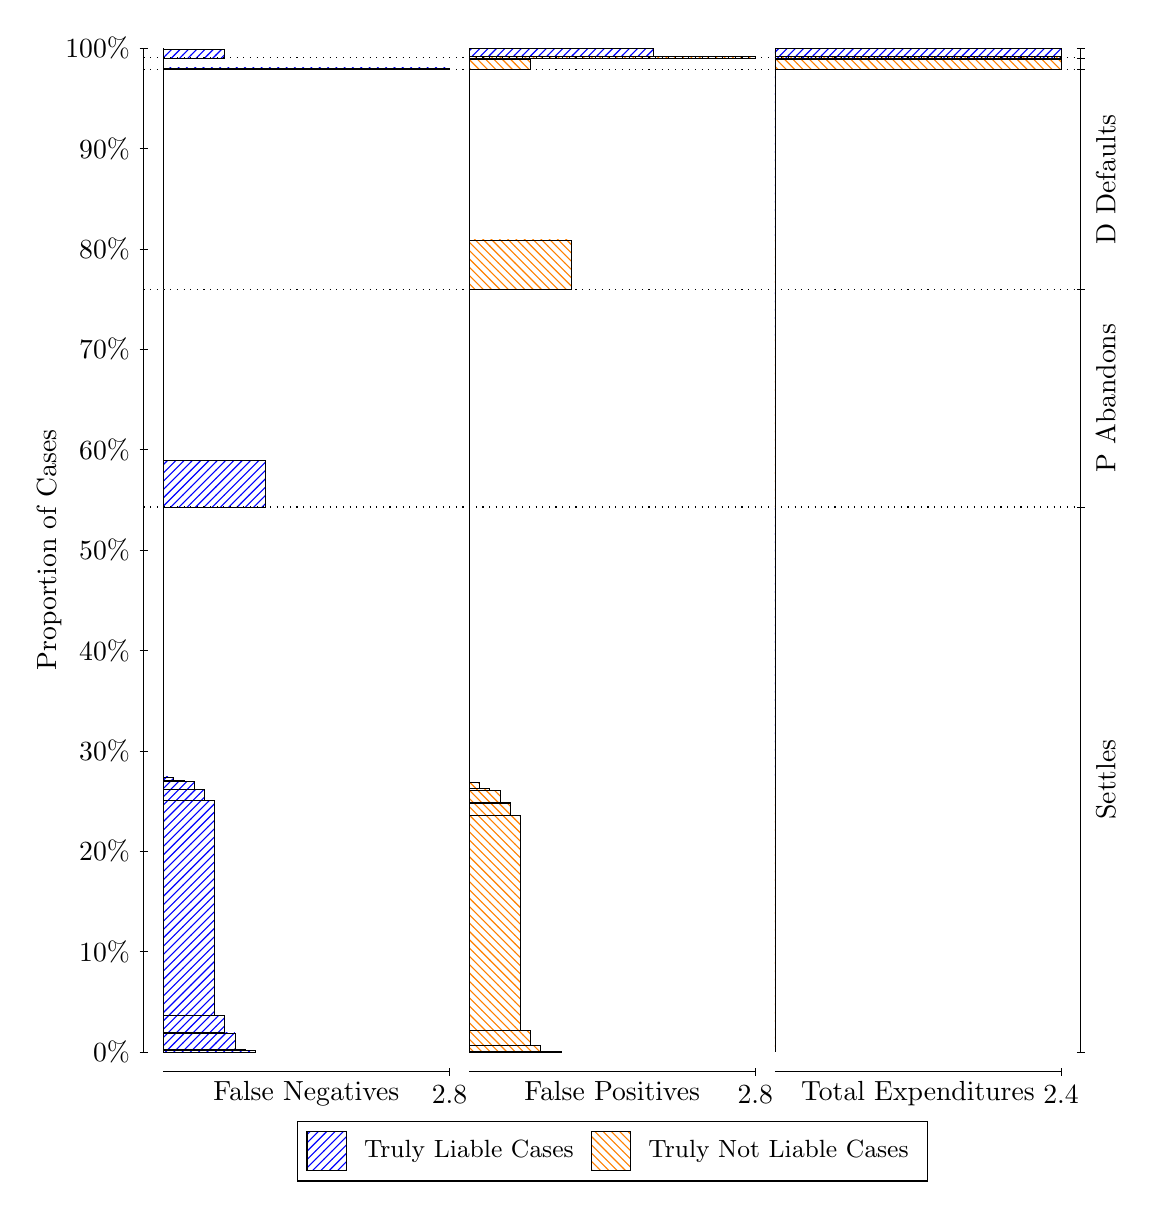
\begin{tikzpicture}
\draw[black, very thin] (1.5,1.75) -- (1.5,14.5);
\node[rotate=90, anchor=center] at (0.3, 8.125) {Proportion of Cases};
\draw[black, very thin] (1.45,1.75) -- (1.55,1.75);
\node[anchor=east] at (1.45, 1.75) {0\%};
\draw[black, very thin] (1.45,3.025) -- (1.55,3.025);
\node[anchor=east] at (1.45, 3.025) {10\%};
\draw[black, very thin] (1.45,4.3) -- (1.55,4.3);
\node[anchor=east] at (1.45, 4.3) {20\%};
\draw[black, very thin] (1.45,5.575) -- (1.55,5.575);
\node[anchor=east] at (1.45, 5.575) {30\%};
\draw[black, very thin] (1.45,6.85) -- (1.55,6.85);
\node[anchor=east] at (1.45, 6.85) {40\%};
\draw[black, very thin] (1.45,8.125) -- (1.55,8.125);
\node[anchor=east] at (1.45, 8.125) {50\%};
\draw[black, very thin] (1.45,9.4) -- (1.55,9.4);
\node[anchor=east] at (1.45, 9.4) {60\%};
\draw[black, very thin] (1.45,10.675) -- (1.55,10.675);
\node[anchor=east] at (1.45, 10.675) {70\%};
\draw[black, very thin] (1.45,11.95) -- (1.55,11.95);
\node[anchor=east] at (1.45, 11.95) {80\%};
\draw[black, very thin] (1.45,13.225) -- (1.55,13.225);
\node[anchor=east] at (1.45, 13.225) {90\%};
\draw[black, very thin] (1.45,14.5) -- (1.55,14.5);
\node[anchor=east] at (1.45, 14.5) {100\%};

\draw[black, very thin] (13.4,1.75) -- (13.4,14.5);
\draw[black, very thin] (13.35,1.75) -- (13.45,1.75);
\node[anchor=west] at (13.35, 1.75) {};
\draw[black, very thin] (13.35,8.6714) -- (13.45,8.6714);
\node[anchor=west] at (13.35, 8.6714) {};
\draw[black, very thin] (13.35,11.435) -- (13.45,11.435);
\node[anchor=west] at (13.35, 11.435) {};
\draw[black, very thin] (13.35,14.226) -- (13.45,14.226);
\node[anchor=west] at (13.35, 14.226) {};
\draw[black, very thin] (13.35,14.375) -- (13.45,14.375);
\node[anchor=west] at (13.35, 14.375) {};
\draw[black, very thin] (13.35,14.5) -- (13.45,14.5);
\node[anchor=west] at (13.35, 14.5) {};

\draw[black, very thin, pattern color=blue, pattern=north east lines] (1.75,1.75) rectangle (2.9179,1.7705);
\draw[black, very thin, pattern color=blue, pattern=north east lines] (1.75,1.7705) rectangle (2.7881,1.7855);
\draw[black, very thin, pattern color=blue, pattern=north east lines] (1.75,1.7855) rectangle (2.6583,1.9911);
\draw[black, very thin, pattern color=blue, pattern=north east lines] (1.75,1.9911) rectangle (2.5286,1.9997);
\draw[black, very thin, pattern color=blue, pattern=north east lines] (1.75,1.9997) rectangle (2.5286,2.2177);
\draw[black, very thin, pattern color=blue, pattern=north east lines] (1.75,2.2177) rectangle (2.3988,4.9431);
\draw[black, very thin, pattern color=blue, pattern=north east lines] (1.75,4.9431) rectangle (2.269,5.0833);
\draw[black, very thin, pattern color=blue, pattern=north east lines] (1.75,5.0833) rectangle (2.1393,5.1821);
\draw[black, very thin, pattern color=blue, pattern=north east lines] (1.75,5.1821) rectangle (2.0095,5.1982);
\draw[black, very thin, pattern color=blue, pattern=north east lines] (1.75,5.1982) rectangle (1.8798,5.2441);
\draw[black, very thin, pattern color=orange, pattern=north west lines] (1.75,5.2441) rectangle (1.75,8.6714);
\draw[black, very thin, pattern color=blue, pattern=north east lines] (1.75,8.6714) rectangle (3.0476,9.2653);
\draw[black, very thin, pattern color=orange, pattern=north west lines] (1.75,9.2653) rectangle (1.75,11.435);
\draw[black, very thin, pattern color=orange, pattern=north west lines] (1.75,11.435) rectangle (1.75,12.064);
\draw[black, very thin, pattern color=blue, pattern=north east lines] (1.75,12.064) rectangle (1.75,14.226);
\draw[black, very thin, pattern color=blue, pattern=north east lines] (1.75,14.226) rectangle (5.3833,14.248);
\draw[black, very thin, pattern color=orange, pattern=north west lines] (1.75,14.248) rectangle (1.75,14.375);
\draw[black, very thin, pattern color=blue, pattern=north east lines] (1.75,14.375) rectangle (2.5286,14.478);
\draw[black, very thin, pattern color=orange, pattern=north west lines] (1.75,14.478) rectangle (1.75,14.5);
\draw[black, very thin, pattern color=orange, pattern=north west lines] (5.6333,1.75) rectangle (6.8012,1.7561);
\draw[black, very thin, pattern color=orange, pattern=north west lines] (5.6333,1.7561) rectangle (6.6714,1.7615);
\draw[black, very thin, pattern color=orange, pattern=north west lines] (5.6333,1.7615) rectangle (6.5417,1.8309);
\draw[black, very thin, pattern color=orange, pattern=north west lines] (5.6333,1.8309) rectangle (6.4119,2.0235);
\draw[black, very thin, pattern color=orange, pattern=north west lines] (5.6333,2.0235) rectangle (6.2821,4.7533);
\draw[black, very thin, pattern color=orange, pattern=north west lines] (5.6333,4.7533) rectangle (6.1524,4.911);
\draw[black, very thin, pattern color=orange, pattern=north west lines] (5.6333,4.911) rectangle (6.1524,4.9202);
\draw[black, very thin, pattern color=orange, pattern=north west lines] (5.6333,4.9202) rectangle (6.0226,5.0746);
\draw[black, very thin, pattern color=orange, pattern=north west lines] (5.6333,5.0746) rectangle (5.8929,5.0951);
\draw[black, very thin, pattern color=orange, pattern=north west lines] (5.6333,5.0951) rectangle (5.7631,5.1773);
\draw[black, very thin, pattern color=blue, pattern=north east lines] (5.6333,5.1773) rectangle (5.6333,8.6714);
\draw[black, very thin, pattern color=orange, pattern=north west lines] (5.6333,8.6714) rectangle (5.6333,10.841);
\draw[black, very thin, pattern color=blue, pattern=north east lines] (5.6333,10.841) rectangle (5.6333,11.435);
\draw[black, very thin, pattern color=orange, pattern=north west lines] (5.6333,11.435) rectangle (6.931,12.064);
\draw[black, very thin, pattern color=blue, pattern=north east lines] (5.6333,12.064) rectangle (5.6333,14.226);
\draw[black, very thin, pattern color=orange, pattern=north west lines] (5.6333,14.226) rectangle (6.4119,14.354);
\draw[black, very thin, pattern color=blue, pattern=north east lines] (5.6333,14.354) rectangle (5.6333,14.375);
\draw[black, very thin, pattern color=orange, pattern=north west lines] (5.6333,14.375) rectangle (9.2667,14.397);
\draw[black, very thin, pattern color=blue, pattern=north east lines] (5.6333,14.397) rectangle (7.969,14.5);
\draw[black, very thin, pattern color=orange, pattern=north west lines] (9.5167,1.75) rectangle (9.5167,5.1773);
\draw[black, very thin, pattern color=blue, pattern=north east lines] (9.5167,5.1773) rectangle (9.5167,8.6714);
\draw[black, very thin, pattern color=orange, pattern=north west lines] (9.5167,8.6714) rectangle (9.5167,10.841);
\draw[black, very thin, pattern color=blue, pattern=north east lines] (9.5167,10.841) rectangle (9.5167,11.435);
\draw[black, very thin, pattern color=orange, pattern=north west lines] (9.5167,11.435) rectangle (9.5167,12.064);
\draw[black, very thin, pattern color=blue, pattern=north east lines] (9.5167,12.064) rectangle (9.5167,14.226);
\draw[black, very thin, pattern color=orange, pattern=north west lines] (9.5167,14.226) rectangle (13.15,14.354);
\draw[black, very thin, pattern color=blue, pattern=north east lines] (9.5167,14.354) rectangle (13.15,14.375);
\draw[black, very thin, pattern color=orange, pattern=north west lines] (9.5167,14.375) rectangle (13.15,14.397);
\draw[black, very thin, pattern color=blue, pattern=north east lines] (9.5167,14.397) rectangle (13.15,14.5);
\draw[black, dotted] (1.5,8.6714) -- (13.4,8.6714);
\draw[black, dotted] (1.5,11.435) -- (13.4,11.435);
\draw[black, dotted] (1.5,14.226) -- (13.4,14.226);
\draw[black, dotted] (1.5,14.375) -- (13.4,14.375);
\draw[black, very thin] (1.75,1.5) -- (5.3833,1.5);
\node[anchor=north] at (3.5667, 1.5) {False Negatives};
\draw[black, very thin] (5.3833,1.45) -- (5.3833,1.55);
\node[anchor=north] at (5.3833, 1.45) {2.8};

\draw[black, very thin] (5.6333,1.5) -- (9.2667,1.5);
\node[anchor=north] at (7.45, 1.5) {False Positives};
\draw[black, very thin] (9.2667,1.45) -- (9.2667,1.55);
\node[anchor=north] at (9.2667, 1.45) {2.8};

\draw[black, very thin] (9.5167,1.5) -- (13.15,1.5);
\node[anchor=north] at (11.333, 1.5) {Total Expenditures};
\draw[black, very thin] (13.15,1.45) -- (13.15,1.55);
\node[anchor=north] at (13.15, 1.45) {2.4};

\node[black, centered, rotate=90] at (13.72, 5.2107) {Settles};
\node[black, centered, rotate=90] at (13.72, 10.053) {P Abandons};
\node[black, centered, rotate=90] at (13.72, 12.83) {D Defaults};



\draw (7.449999999999999,1.5) node[draw=none] (baseCoordinate) {};
\begin{scope}[align=center]
        \matrix[scale=0.5, draw=black, below=0.5cm of baseCoordinate, nodes={draw}, column sep=0.1cm]{
            \node[rectangle, draw, minimum width=0.5cm, minimum height=0.5cm, pattern=north east lines, pattern color=blue] {}; &
            \node[draw=none, font=\small] (B) {Truly Liable Cases}; &
            \node[rectangle, draw, minimum width=0.5cm, minimum height=0.5cm, pattern=north west lines, pattern color=orange] {}; &
            \node[draw=none, font=\small] (B) {Truly Not Liable Cases}; \\
            };
\end{scope}

\end{tikzpicture}
\end{document}